\documentclass[border=3pt]{standalone}
\usepackage{mathptmx}
\usepackage{amsmath}
\usepackage{tikz}
\usetikzlibrary{arrows.meta,calc,decorations.pathreplacing}
\begin{document}
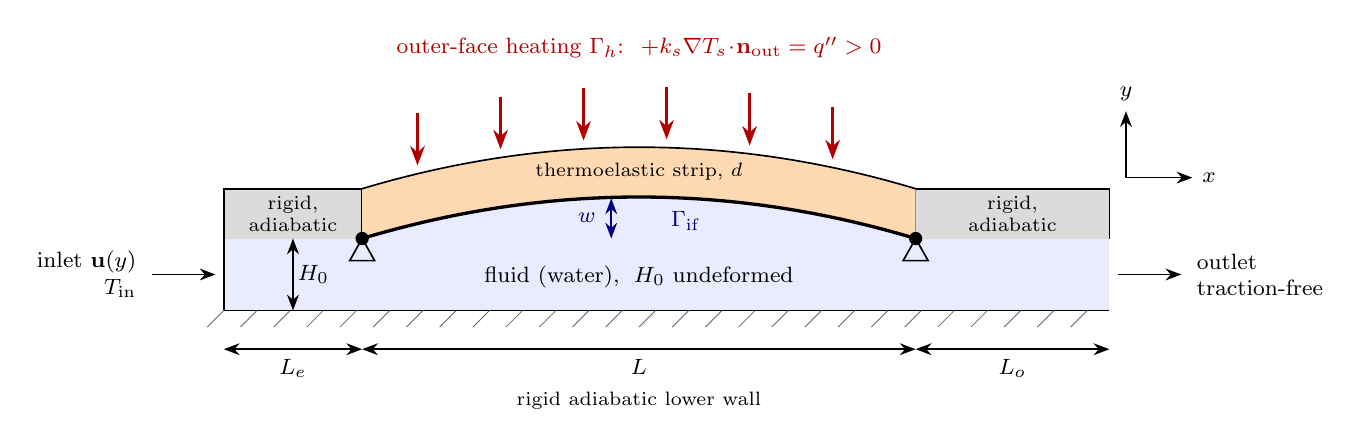
\begin{tikzpicture}[x=1pt,y=1pt,>=Stealth,font=\footnotesize,line width=0.6pt]
% ---------- scaled layout (heights exaggerated); not to scale ----------
\def\Le{50}\def\L{200}\def\Lo{70}      % entrance, heated segment, exit
\def\Hf{26}                            % channel height H_0 (exaggerated)
\def\ds{18}                            % wall thickness d (exaggerated)
\def\bow{15}                           % mid-span bow (exaggerated)
% fluid
\fill[blue!8] (0,0) rectangle (\Le+\L+\Lo,\Hf);
% fluid beneath the bowed strip (passage widens)
\fill[blue!8] (\Le,\Hf) .. controls (\Le+\L/3,\Hf+4/3*\bow) and (\Le+2*\L/3,\Hf+4/3*\bow) .. (\Le+\L,\Hf) -- cycle;
% rigid upper sections (casing), grey
\fill[black!14] (0,\Hf) rectangle (\Le,\Hf+\ds);
\fill[black!14] (\Le+\L,\Hf) rectangle (\Le+\L+\Lo,\Hf+\ds);
\draw (0,\Hf) -- (0,\Hf+\ds) -- (\Le,\Hf+\ds) -- (\Le,\Hf);
\draw (\Le+\L,\Hf) -- (\Le+\L,\Hf+\ds) -- (\Le+\L+\Lo,\Hf+\ds) -- (\Le+\L+\Lo,\Hf);
% bowed thermoelastic strip (both faces displaced upwards by w)
\fill[orange!30] (\Le,\Hf) .. controls (\Le+\L/3,\Hf+4/3*\bow) and (\Le+2*\L/3,\Hf+4/3*\bow) .. (\Le+\L,\Hf)
  -- (\Le+\L,\Hf+\ds) .. controls (\Le+2*\L/3,\Hf+\ds+4/3*\bow) and (\Le+\L/3,\Hf+\ds+4/3*\bow) .. (\Le,\Hf+\ds) -- cycle;
\draw[very thick] (\Le,\Hf) .. controls (\Le+\L/3,\Hf+4/3*\bow) and (\Le+2*\L/3,\Hf+4/3*\bow) .. (\Le+\L,\Hf);
\draw (\Le,\Hf+\ds) .. controls (\Le+\L/3,\Hf+\ds+4/3*\bow) and (\Le+2*\L/3,\Hf+\ds+4/3*\bow) .. (\Le+\L,\Hf+\ds);
% channel walls
\draw (0,0) -- (\Le+\L+\Lo,0);
\draw (0,\Hf) -- (0,0);
% lower wall hatch
\foreach \x in {0,12,...,\numexpr\Le+\L+\Lo\relax}{\draw[black!60,line width=0.3pt] (\x,0) -- (\x-6,-6);}
% heater arrows on outer face
\foreach \t in {0.10,0.25,0.40,0.55,0.70,0.85}{
  \pgfmathsetmacro{\xx}{\Le+\t*\L}
  \pgfmathsetmacro{\yy}{\Hf+\ds+4*\bow*\t*(1-\t)}
  \draw[->,red!70!black,line width=0.9pt] (\xx,\yy+22) -- (\xx,\yy+3);}
\node[red!70!black] at (\Le+\L/2,\Hf+\ds+\bow+36) {outer-face heating $\Gamma_h$:\; $+k_s\nabla T_s\!\cdot\!\mathbf{n}_{\mathrm{out}}=q''>0$};
% interface label and deflection arrow
\node[blue!50!black,anchor=north west,align=left] at (\Le+\L/2+8,\Hf+\bow*0.9) {$\Gamma_{\mathrm{if}}$};
\draw[<->,blue!50!black] (\Le+\L/2-10,\Hf) -- (\Le+\L/2-10,\Hf+\bow-0.5);
\node[blue!50!black,anchor=east] at (\Le+\L/2-12,\Hf+\bow/2) {$w$};
\node[align=center,font=\scriptsize] at (\Le+\L/2,\Hf+\ds/2+\bow) {thermoelastic strip, $d$};
% fluid labels
\node[align=center] at (\Le+\L/2,\Hf/2-1) {fluid (water),\; $H_0$ undeformed};
% inlet / outlet
\draw[->] (-26,\Hf/2) -- (-3,\Hf/2);
\node[anchor=east,align=right] at (-28,\Hf/2) {inlet $\mathbf{u}(y)$\\$T_{\mathrm{in}}$};
\draw[->] (\Le+\L+\Lo+3,\Hf/2) -- (\Le+\L+\Lo+26,\Hf/2);
\node[anchor=west,align=left] at (\Le+\L+\Lo+28,\Hf/2) {outlet\\ traction-free};
% pins
\foreach \px in {\Le,\Le+\L}{ \fill[black] (\px,\Hf) circle (2.4pt);
  \draw (\px,\Hf) -- ++(-4.5,-8) -- ++(9,0) -- cycle;}
% dimensions
\draw[<->] (0,-14) -- (\Le,-14) node[midway,below] {$L_e$};
\draw[<->] (\Le,-14) -- (\Le+\L,-14) node[midway,below] {$L$};
\draw[<->] (\Le+\L,-14) -- (\Le+\L+\Lo,-14) node[midway,below] {$L_o$};
\draw[<->] (\Le/2,0) -- (\Le/2,\Hf) node[midway,right,inner sep=1.5pt] {$H_0$};
% grey region labels
\node[font=\scriptsize,align=center] at (\Le/2,\Hf+\ds/2) {rigid,\\adiabatic};
\node[font=\scriptsize,align=center] at (\Le+\L+\Lo/2,\Hf+\ds/2) {rigid,\\adiabatic};
\node[font=\scriptsize,anchor=north] at (\Le+\L/2,-26) {rigid adiabatic lower wall};
% axes
\draw[->] (\Le+\L+\Lo+6,\Hf+\ds+4) -- ++(24,0) node[right] {$x$};
\draw[->] (\Le+\L+\Lo+6,\Hf+\ds+4) -- ++(0,24) node[above] {$y$};
\end{tikzpicture}
\end{document}
